\documentclass[border=7pt]{standalone}
\usepackage{tkz-euclide}
\usetkzobj{all} % on charge tous les objets
\usetikzlibrary{decorations.pathreplacing}

\begin{document}
  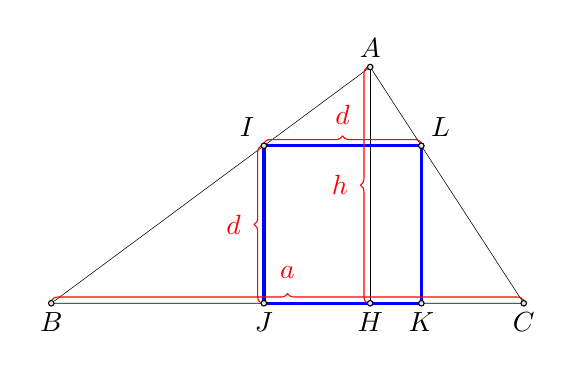
\begin{tikzpicture}
    \clip (-4,-.5) rectangle (2.5,3.5);
    % définition des points
    \tkzDefPoints{-1/0/J,1/0/K}
    \tkzDefSquare(J,K) \tkzGetPoints{L}{I}
    \tkzDefPoint(.35,3){A}
    \tkzInterLL(A,I)(J,K) \tkzGetPoint{B}
    \tkzInterLL(A,L)(J,K) \tkzGetPoint{C}
    \tkzDefPointsBy[projection=onto B--C](A){H}
    % tracer
    \tkzDrawPolygon(A,B,C)
    \tkzDrawSegment(A,H)
    \tkzDrawPolygon[very thick,blue](I,J,K,L)
    % les longueurs
    \begin{scope}[len/.style={red, decorate,decoration={brace,raise=1pt}}]
      \draw[len] (J) -- (I) node [midway,xshift=-11pt]{$d$};
      \draw[len] (H) -- (A) node [midway,xshift=-11pt]{$h$};
      \draw[len] (I) -- (L) node [midway,yshift=11pt]{$d$};
      \draw[len] (B) -- (C) node [midway,yshift=11pt]{$a$};
    \end{scope}
    % marquage des points
    \tkzDrawPoints(A,B,C,H,I,J,K,L)
    \tkzLabelPoints[above](A)
    \tkzLabelPoints[below](B,J,H,K,C)
    \tkzLabelPoints[above left](I)
    \tkzLabelPoints[above right](L)
  \end{tikzpicture}
\end{document}
